This chapter will describe the requirements of the application as a whole. The structure of this chapter roughly follows the SRS Template suggested by [reference: Software Requirements, by Karl E Wiegers and Joy Beatty]

\section{Vision and Scope}

    \subsection{Background}

        Melanoma is a type malignant skin tumour that develops from benign melanocytic nevi. Although less frequent than other skin cancer types, it causes more deaths [http://www.cancer.gov/types/skin], and it’s incidence is increasing dramatically, especially in the young white population [reference: Pattern Analysis in Dermoscopic Images , Aurora Sáez ]. Early diagnosis and treatment is vital.

Several non-invasive techniques exist which dermatologist can employ to visually make a diagnosis. The most common are pattern analysis, the ABCD rule, the 7-point checklist and the Menzies method, among others [reference: An Atlas of Dermoscopy edited by Ashfaq A Marghoob, Josep Malvehy, Ralph P Braun, Alfred W. Kopf]. These methods generally use a combination of defined visual clues and indicators to assess the risk of a skin lesion. CAD ( Computer Aided Diagnosis ) systems exists that can assist a dermatologist, and even provide automatic diagnosis with an accuracy comparable to that of doctors trained in dermoscopic techniques. [reference : A Review of the Quantification and Classification of Pigmented Skin Lesions: From Dedicated to Hand-Held Devices , Mercedes Filho, Zhen Ma and João Manuel R. S. Tavares ]

    \subsection{Business Case}

        A smart phone based assistant would provide a valuable service by making it easy, painless, inexpensive, and fast to get a preliminary risk assessment of a skin lesion. It is too easy to postpone making an appointment with a dermatologist to have a suspect lesion examined. Visiting an dermatologist is not on most people’s list of fun things to do in the spare time, it requires time and effort. By the time a lesion is visually compelling enough, it might be too late.

A smart phone based application that could make a preliminary diagnosis in near real time would be a great time save and offer compelling enough information to actually make the appointment with a dermatologist.

    \subsection{Scope and Limitations}
    \subsubsection{Major Features}
        \noindent
        \begin{itemize}[leftmargin=*]
            \item[]  \textbf{FE-1} : The smart phone app allows the user to capture and analyse an image of a skin lesion and provide a risk assessment to the user of the lesion being a malignant melanoma.

            \item[] \textbf{FE-2} : The app allows the user to create, view, edit or delete metadata that is associated with an image and corresponding risk assessment.

            \item[] \textbf{FE-3} : The app allows the user to save or archive the image and corresponding assessment for future comparison and review.

            \item[] \textbf{FE-4} : The user can browse archived images, assessments, and associated metadata.

            \item[] \textbf{FE-5} : The user can send a set of images with associated assessment and metadata via email.

            \item[] \textbf{FE-6} : The app will run on all popular smart phone devices and systems.

            \item[] \textbf{FE-7} : The analysis algorithms employed by the app should be easily updatable and extendable.
        \end{itemize}

        \begin{figure}[H]
            \centering
            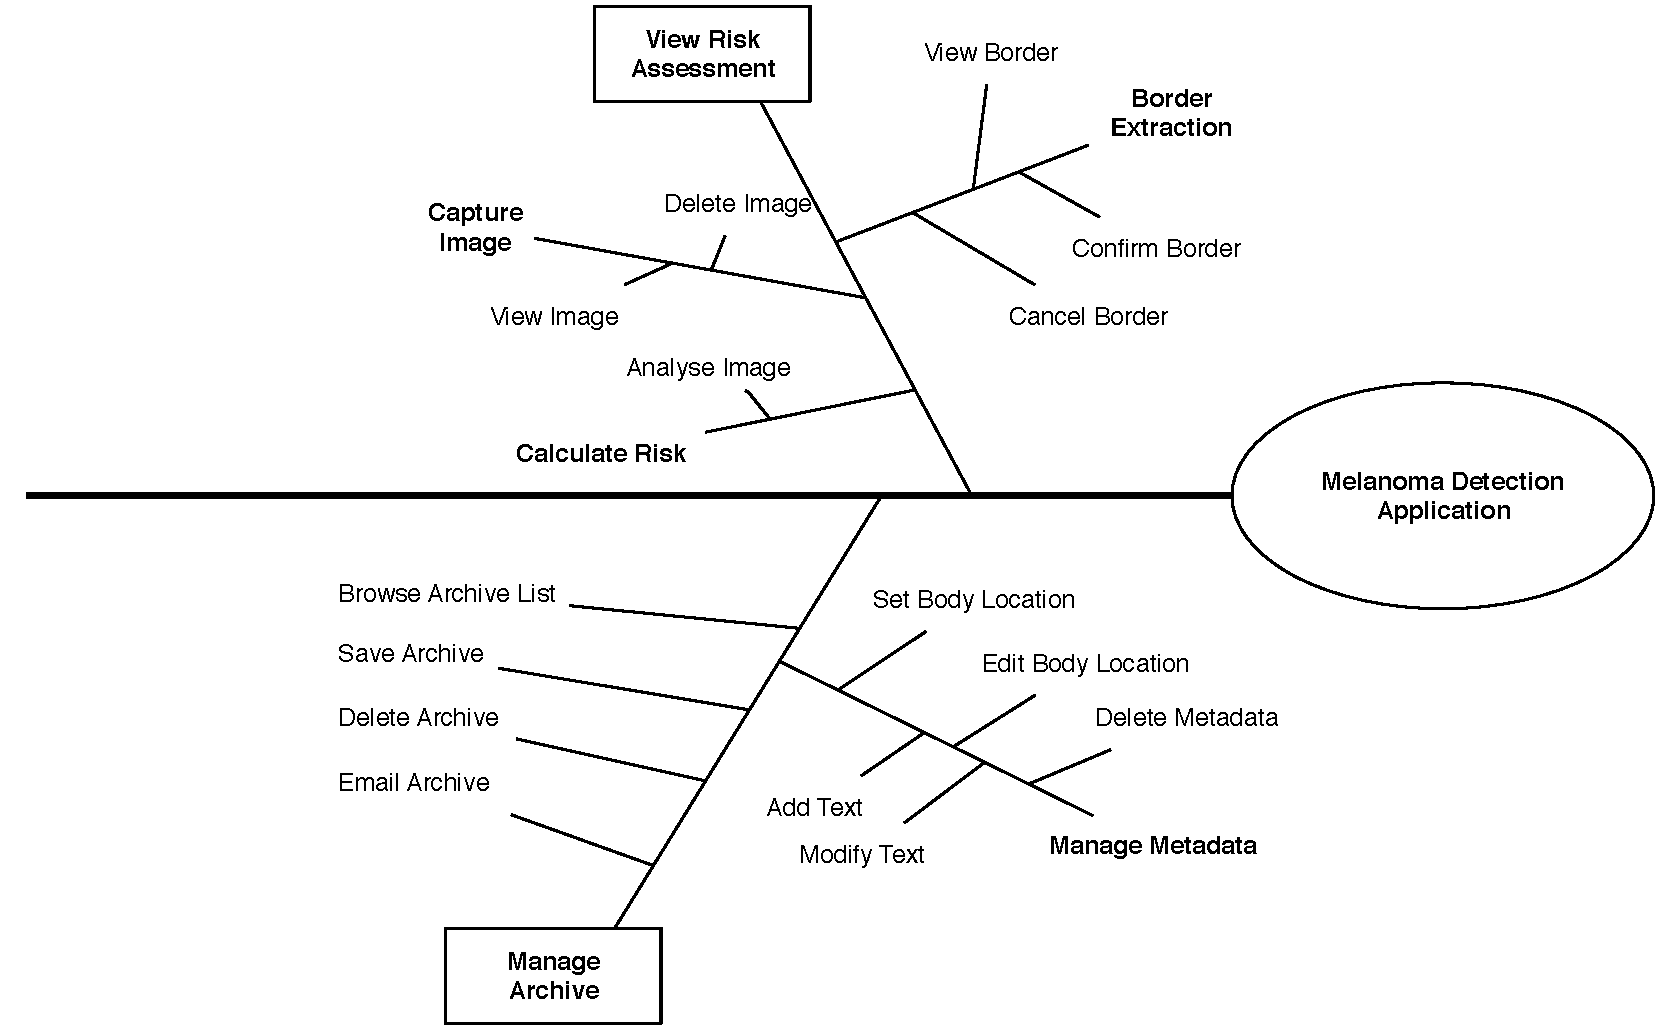
\includegraphics[width=\textwidth]{assets/requirements/PartialFeatureTree.pdf}
            \caption{Partial Feature Tree for the Melanoma Detection App}
            \label{fig:partial_feature_tree}
        \end{figure}


    \subsubsection{Limitations and Exclusions}
    \subsubsection{Business Context}
    \subsection{Use Cases}

        \begin{figure}[H]
            \centering
            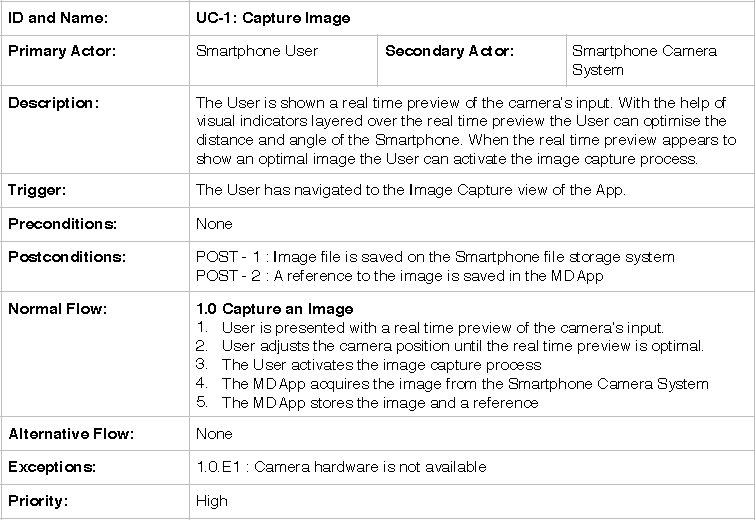
\includegraphics[width=\textwidth]{assets/requirements/uc/usecase_01.pdf}
            \caption{UC-1}
            \label{fig:uc-1}
        \end{figure}
        \begin{figure}[H]
            \centering
            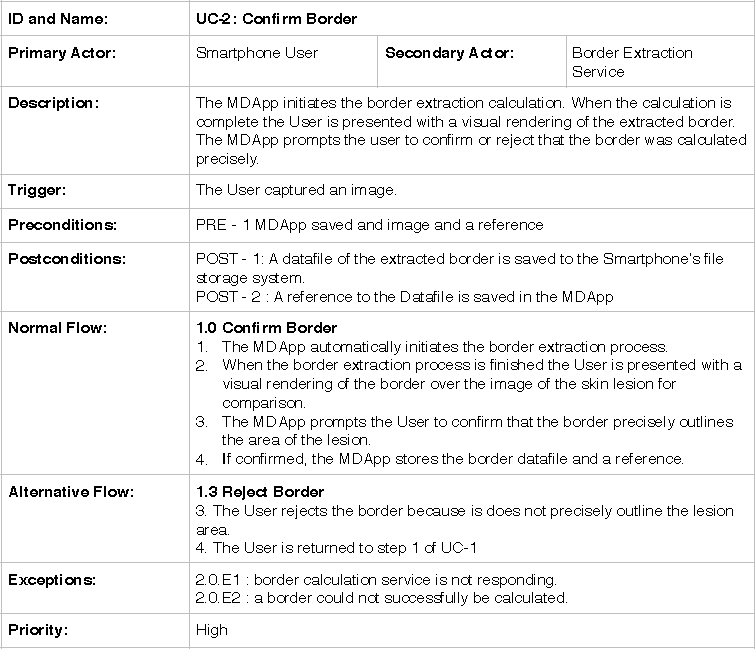
\includegraphics[width=\textwidth]{assets/requirements/uc/usecase_02.pdf}
            \caption{UC-2}
            \label{fig:uc-2}
        \end{figure}
        \begin{figure}[H]
            \centering
            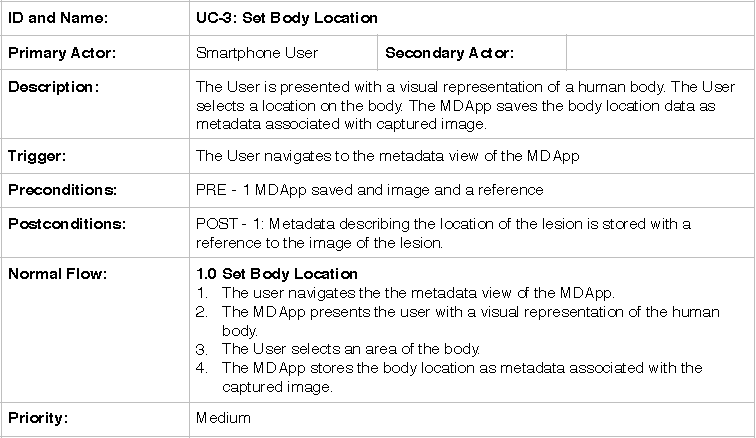
\includegraphics[width=\textwidth]{assets/requirements/uc/usecase_03.pdf}
            \caption{UC-3}
            \label{fig:uc-3}
        \end{figure}
        \begin{figure}[H]
            \centering
            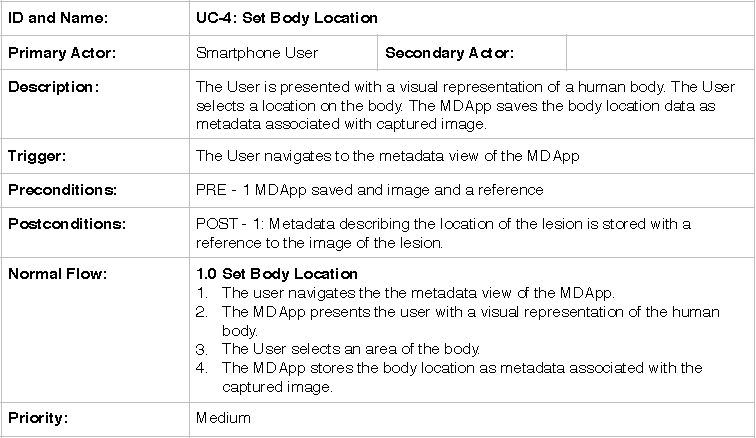
\includegraphics[width=\textwidth]{assets/requirements/uc/usecase_04.pdf}
            \caption{UC-4}
            \label{fig:uc-4}
        \end{figure}
        \begin{figure}[H]
            \centering
            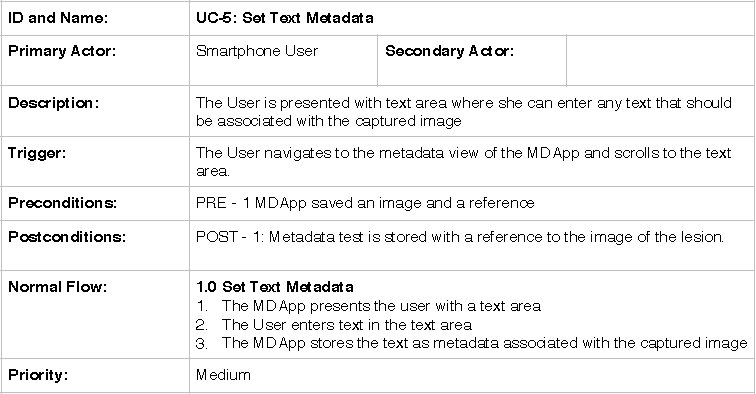
\includegraphics[width=\textwidth]{assets/requirements/uc/usecase_05.pdf}
            \caption{UC-5}
            \label{fig:uc-5}
        \end{figure}
        \begin{figure}[H]
            \centering
            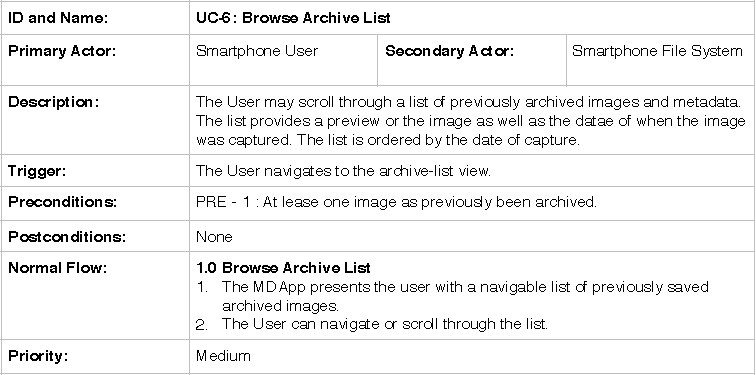
\includegraphics[width=\textwidth]{assets/requirements/uc/usecase_06.pdf}
            \caption{UC-6}
            \label{fig:uc-6}
        \end{figure}
        \begin{figure}[H]
            \centering
            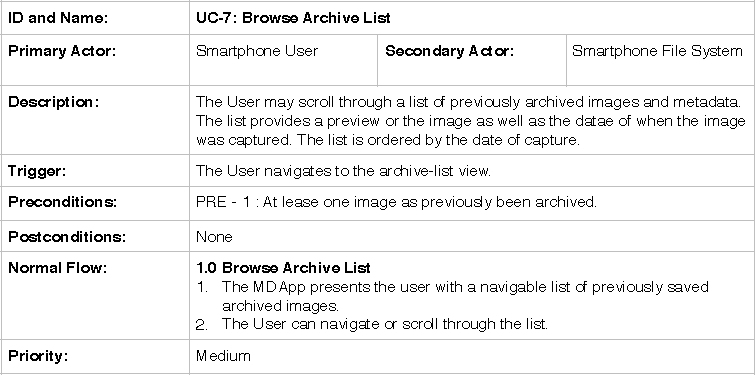
\includegraphics[width=\textwidth]{assets/requirements/uc/usecase_07.pdf}
            \caption{UC-7}
            \label{fig:uc-7}
        \end{figure}
        \begin{figure}[H]
            \centering
            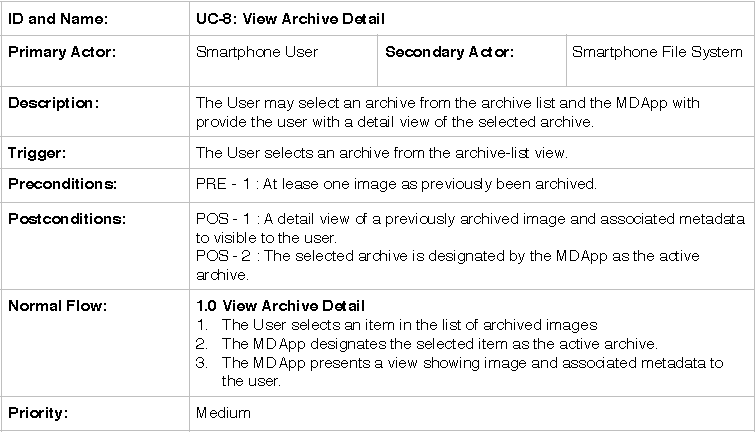
\includegraphics[width=\textwidth]{assets/requirements/uc/usecase_08.pdf}
            \caption{UC-8}
            \label{fig:uc-8}
        \end{figure}

\section{Software Requirements Specification}

    \subsection{Introduction}

    \subsection{Overall Description}

        \subsubsection{Product Perspective}


            \begin{figure}[H]
                \centering
                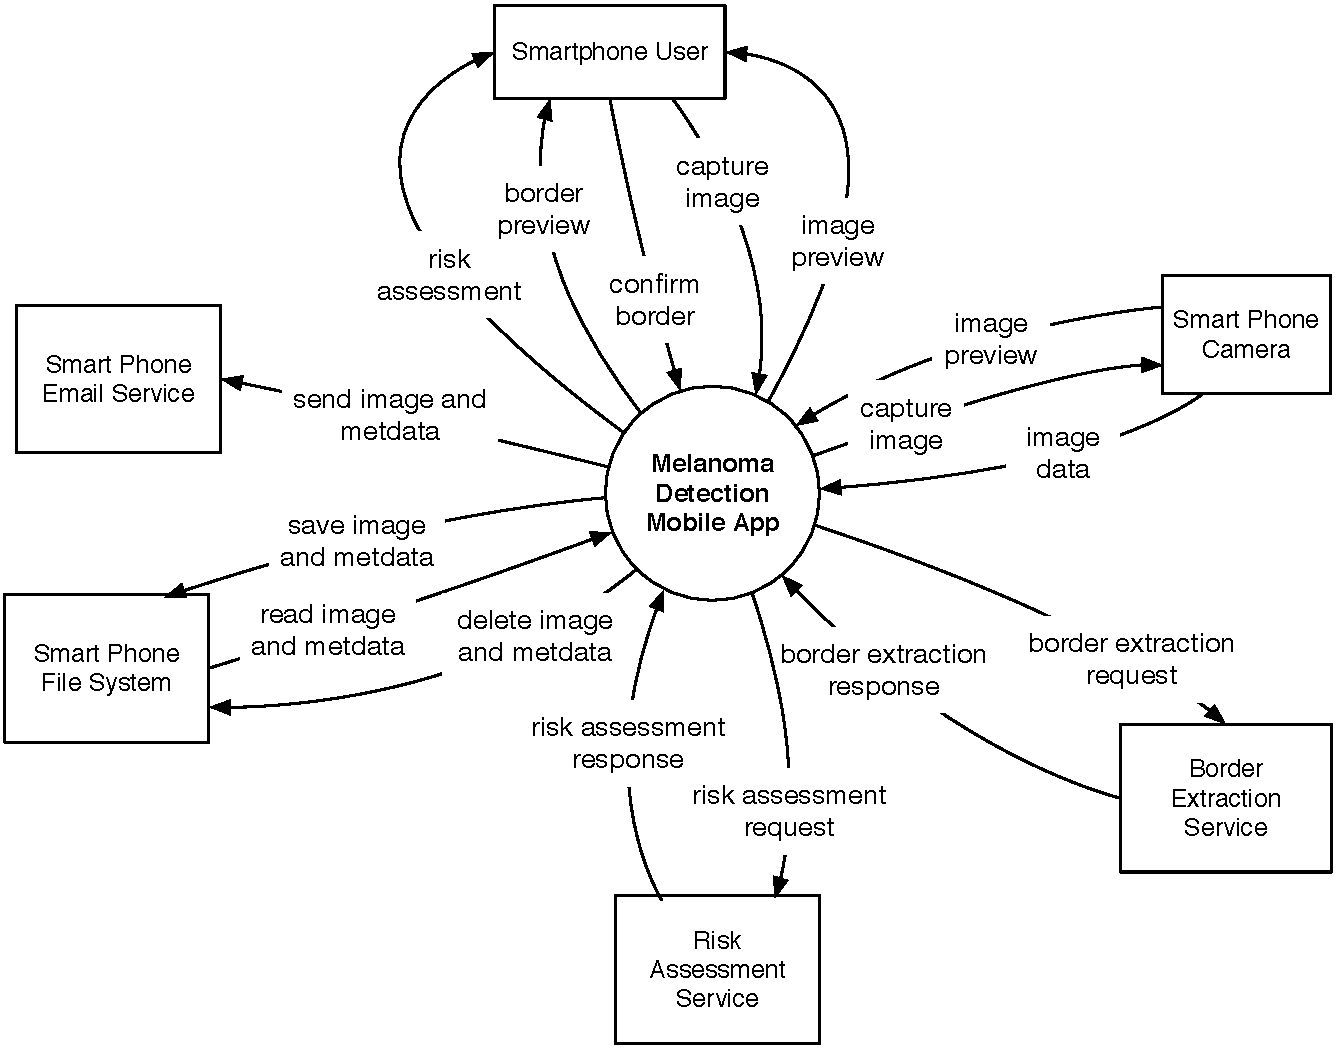
\includegraphics[width=\textwidth]{assets/requirements/ContextDiagram.pdf}
                \caption{Context Diagram of the Melanoma Detection App}
                \label{fig:partial_feature_tree}
            \end{figure}


        \subsubsection{User Classes and Characteristics}
        \subsubsection{Operating Environment}
        \subsubsection{Design and Implementation Constraints}
        \subsubsection{Assumptions and Dependencies}

    \subsection{System Features}

        \subsubsection{Capture Image}
            \paragraph{Description}
            \paragraph{Functional Requirements}

        \subsubsection{Calculate Border}
            \paragraph{Description}
            \paragraph{Functional Requirements}

    \subsection{Data Requirements}
        \subsubsection{Logical Data Model}
        \subsubsection{Data Dictionary}
        \subsubsection{Reports}






